%!TEX root = slides.tex

\title{Theory of Algorithms}
\subtitle{}
\author{ian.mcloughlin@gmit.ie}
\date{}


\begin{frame}
	\titlepage
\end{frame}

\begin{frame}
	\frametitle{Topics}
	\tableofcontents
\end{frame}

\section{Python}


\begin{frame}{About Python}
  \begin{description}
    \item[January 1994] -- Python 1.0.0 released.
    \vspace{0.25cm}
    \item[Guido van Rossum] -- Designer/Author of Python.
    \vspace{0.25cm}
    \item[Current versions] -- 3.5.1 and 2.7.11.
    \vspace{0.25cm}
    \item[Interpreted] -- Python implementation must be present at runtime.
    \vspace{0.25cm}
    \item[Off-side rule] -- Blocks identified by indentation, as opposed to curly braces.
    \vspace{0.25cm} 
    \item[Popularity] -- IEEE Spectrum ranks it as the fourth most popular language (July 2015).
    \vspace{0.25cm}
    \item[Community] -- Python Enhancement Proposals, notably \href{https://www.python.org/dev/peps/pep-0008/}{PEP 8: The Python Style Guide}.
    \vspace{0.25cm} 
  \end{description}
  \citeurl{spectrum.ieee.org/computing/software/the-2015-top-ten-programming-languages}
\end{frame}


\begin{frame}{Guido van Rossum}
  \begin{columns}
    \begin{column}{0.2\textwidth}
      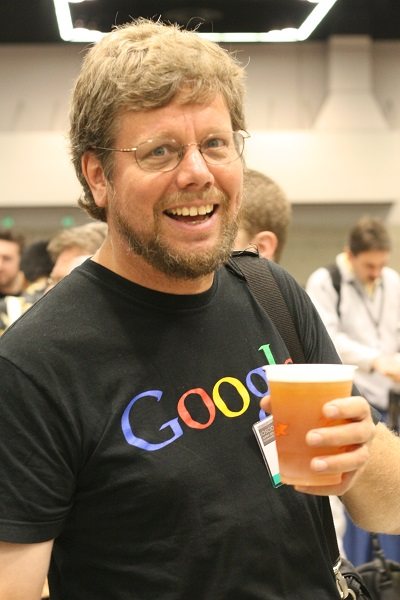
\includegraphics[height=2in]{img/guido_van_rossum.jpg}
    \end{column}
    \begin{column}{0.6\textwidth}
      \begin{itemize}
    		\item Started Python as a hobby.
        \vspace{0.25cm}
    		\item Worked for Google, half-time spent on Python.
        \vspace{0.25cm}
    		\item Now works at Dropbox.
        \vspace{0.25cm}
        \item Benevolent dictator for life (BDFL).
      \end{itemize}
    \end{column}
  \end{columns}
\end{frame}

\begin{frame}[fragile]{Conditions}
  \begin{minted}[linenos, frame=lines, framesep=2mm]{python}
x = int(raw_input("Please enter an integer: "))
if x < 0:
  x = 0
  print 'Negative changed to zero'
elif x == 0:
  print 'Zero'
elif x == 1:
  print 'Single'
else:
  print 'More'
  \end{minted}
  \citeurl{docs.python.org/2/tutorial}
\end{frame}

\begin{frame}[fragile]{Loops}
  \begin{minted}[linenos, frame=lines, framesep=2mm]{python}
# A for loop.
a = ['Mary', 'had', 'a', 'little', 'lamb']
for i in range(len(a)):
  print i, a[i]
  \end{minted}
  \begin{minted}[linenos, frame=lines, framesep=2mm]{python}
# A while loop.
a, b = 0, 1
while b < 1000:
  print b,
  a, b = b, a+b
  \end{minted}
  \citeurl{docs.python.org/2/tutorial}
\end{frame}

\begin{frame}[fragile]{Functions}
  \begin{minted}[linenos, frame=lines, framesep=2mm]{python}
# write Fibonacci series up to n
def fib(n):   
  """Print a Fibonacci series up to n."""
  a, b = 0, 1
  while a < n:
    print a,
    a, b = b, a+b
  \end{minted}
  \citeurl{docs.python.org/2/tutorial}
\end{frame}

\begin{frame}{CPython}
  \begin{description}
    \item[Reference implementation] -- Many different Python implementations exist.
    \vspace{0.25cm}
    \item[Version 3] -- Broke backwards compatibility (somewhat).
    \vspace{0.25cm}
    \item[Unladen Swallow] -- Google attempt to fix some Python problems.
    \vspace{0.25cm}
    \item[Modules] -- Lots of great Python modules available.
  \end{description}
  \citeurl{www.python.org}
\end{frame}


\section{Timing Algorithms}

\section{Functional Programming}

\section{Turing Machines}

\section{Complexity Classes}